% !TEX root = ../main.tex
% Хавсралт Д

\chapter{Хугарлын зэрэг үнэлгээний жишээ}
\label{AppendixE}
\pagecolor{white}

Хугарлын сегментчлэлийн үр дүнд үндэслэн морфологийн шинжүүдийг гарган авч үнэлгээ хийсэн. Хүснэгт~\ref{tab:appE_geom}-д нэг жишээ тохиолдол (Grade~2)-д тооцоолсон геометрийн шинжүүдийг үзүүлэв. (Grade зургууд болон бодит шинжийн утгыг \texttt{appendix\_scripts/gen\_E\_severity.py} script-ээр үүсгэнэ.)

\begin{table}[ht]
    \centering
    \begin{tabular}{|l|c|}
    \hline
    \textbf{Үзүүлэлт} & \textbf{Утга} \\ \hline
    Area (талбай, px$^2$)         & 1{,}872 \\ \hline
    Major axis (гол тэнхлэг, px)  & 55.41 \\ \hline
    Aspect Ratio (тал харьцаа)    & 1.23 \\ \hline
    Solidity (нягтрал)            & 1.00 \\ \hline
    Severity Score (зэргийн оноо) & 2 (Grade~2) \\ \hline
    \end{tabular}
    \caption{Геометрийн шинжүүдийн жишээ (\texttt{gen\_E\_severity.py}-ийн сонгосон Grade~2 тохиолдол)}
    \label{tab:appE_geom}
\end{table}

\begin{figure}[H]
    \centering
    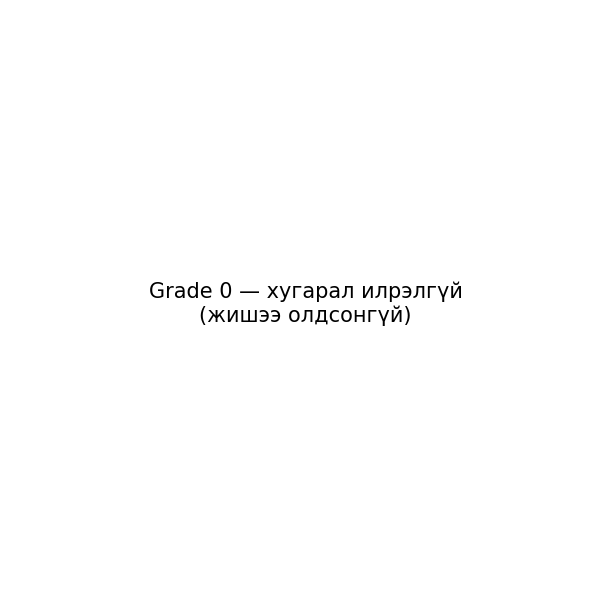
\includegraphics[width=0.48\textwidth,height=0.48\textheight,keepaspectratio]{Figures/appx_e_grade0.png}
    \figcaption{Grade 0}{Grade 0}
    \label{fig:appE_g0}
\end{figure}

\begin{figure}[H]
    \centering
    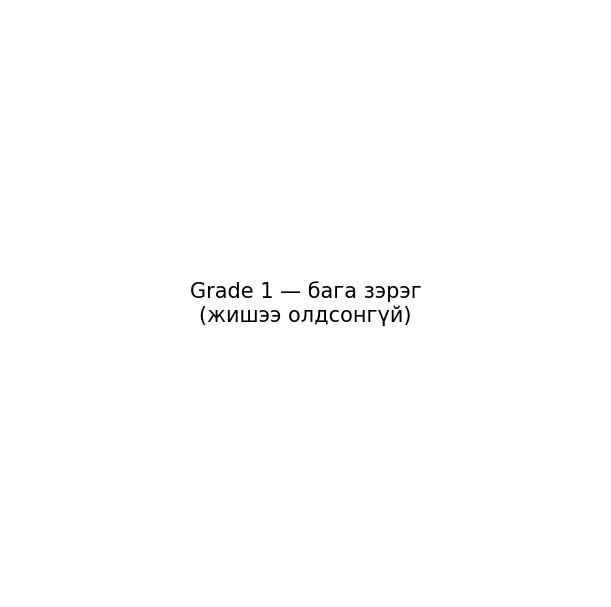
\includegraphics[width=0.48\textwidth,height=0.48\textheight,keepaspectratio]{Figures/appx_e_grade1.png}
    \figcaption{Grade 1}{Grade 1}
    \label{fig:appE_g1}
\end{figure}

\begin{figure}[H]
    \centering
    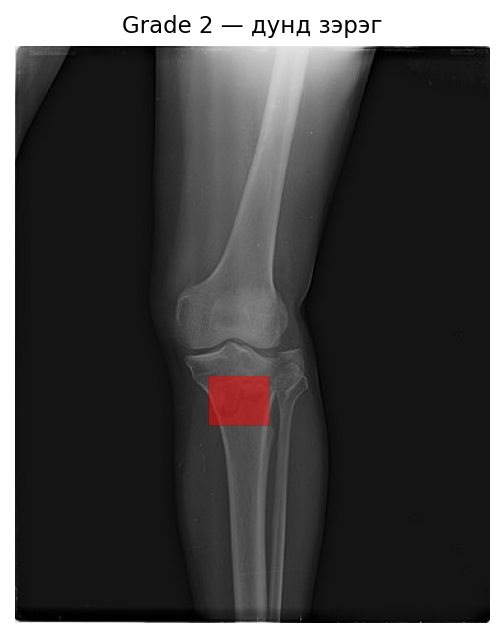
\includegraphics[width=0.45\textwidth,height=0.48\textheight,keepaspectratio]{Figures/appx_e_grade2.png}
    \figcaption{Grade 2}{Grade 2}
    \label{fig:appE_g2}
\end{figure}

\begin{figure}[H]
    \centering
    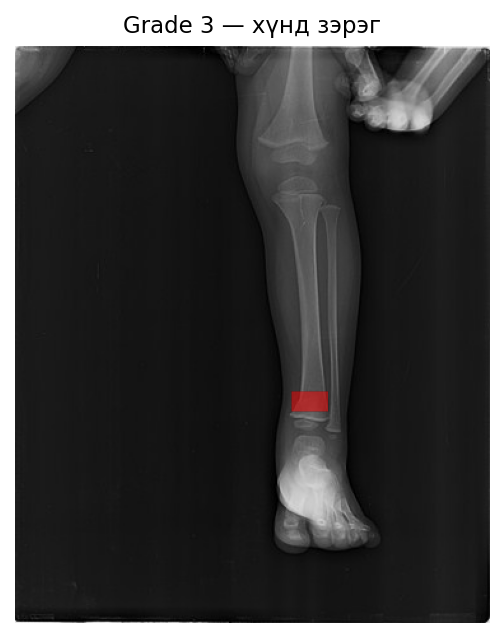
\includegraphics[width=0.45\textwidth,height=0.48\textheight,keepaspectratio]{Figures/appx_e_grade3.png}
    \figcaption{Grade 3}{Grade 3}
    \label{fig:appE_g3}
\end{figure}
